\documentclass[12pt]{article}

\usepackage[spanish]{babel}
\usepackage{hyperref}
\usepackage{graphicx}
\usepackage{listings}
\usepackage{color}
\usepackage{multicol}
\usepackage{amssymb}
\usepackage{enumitem}
\usepackage{here}
\usepackage{dsfont}
\usepackage{amsmath}
\usepackage{tipa}
\usepackage{float}
\spanishdecimal{.}

\title{Matemáticas para las Ciencias Aplicadas I}
\title{
	Cuarta Lista de Problemas \\
	\textbf{Primera  Parte} \\
	\vspace{1ex}
	\large Matemáticas para las Ciencias Aplicadas I \\
	Facultad de Ciencias, UNAM}

\date{\today}

\author{Flores Morán Julieta Melina \\ Zarco Romero José Antonio}

%% Sección 5.3: 44 y 73.
%% Sección 5.5: 28 y 37.
%% Sección 5.6: 58, 63 y 70.
%% Sección 5.8: 27.
%% Sección 5.9: 52 y 64

\begin{document}

\maketitle

%% 5.3 -----------------------------------------------------------------------------------------------------------------------------------------------------------------------------------------------------------------------------
\section{Sección 5.3 \\ Integración Por Sustitución}
% 44 -------------------------------------------------------------------------------------------------------------
\subsection{Ejercicio 44} Flores Morán Julieta Melina \\

Evaluar las integrales utilizando sustituciones apropiadas.
\[
\int \tan^3{5x}\sec^2{5x}dx
\]
Tomemos $u=\tan{5x} \rightarrow du = 5 \sec^{2}5xdx \rightarrow \frac{du}{5} = \sec^{2}5xdx $. \\
Sustituimos en la integral:
\[
\int u^3 \frac{du}{5}
\]
Y resolvemos normalmente:\\
\begin{align*}
  \int u^3 \frac{du}{5}
  & = \int u^3 du \frac{1}{5} \\
  & = \frac{1}{5} \int u^3 du \\
  & = \frac{1}{5} \frac {u^4}{4} + C \\
  & = \frac {u^4}{20} + C\\
\end{align*}
y regresamos a u a su valor original.
\begin{align*}
  \frac {u^4}{20} + C 
  & = \frac{\tan^45x}{20} + C
\end{align*}
% 73 -------------------------------------------------------------------------------------------------------------
\subsection{Ejercicio 73} Zarco Romero José Antonio \\

\begin{enumerate}[label=(\alph*)]
  
\item Evalúe $\int \left[ \frac {x}{\sqrt{x^2+1}}  \right] dx$

  Si hacemos que $u = x^2+1$, entonces
  
  \[
  \frac{du}{dx}=2x \qquad \text{ así, } \qquad \frac{du}{2}=xdx
  \]

  De este modo,

  \begin{align*}
    \int \left[ \frac {x}{\sqrt{x^2+1}}  \right] dx
    &= \int \left[ \frac {1}{2} u^{-\frac{1}{2}}  \right] du \\
    &= \frac {1}{2} \int u^{-\frac{1}{2}} du \\
    &=  \frac {1}{2} \left[ 2u^{\frac{1}{2}} \right] + C \\
    &= u^{\frac{1}{2}} +C \\
    &= \sqrt{x^2+1} +C
  \end{align*}

\item Utilice una herramienta gráfica para generar algunas curvas integrales típicas de $f(x) = x / \sqrt{x^2 + 1}$ en el intervalo $(-5, 5)$.

  \begin{figure}[H]
       \centering
       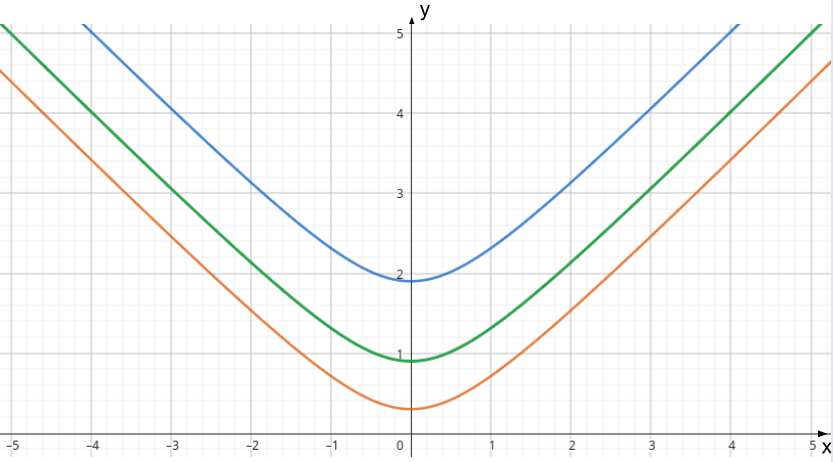
\includegraphics[width=1\textwidth]{../img/img_Lista4/1_73_b.png}
  \end{figure}
  
\end{enumerate}

%% 5.5 -----------------------------------------------------------------------------------------------------------------------------------------------------------------------------------------------------------------------------
\section{Sección 5.5 \\ La Integral Definida}
% 28 -------------------------------------------------------------------------------------------------------------
\subsection{Ejercicio 28} Flores Morán Julieta Melina \\

Utilice el Teorema 5.5.4 y fórmulas apropiadas de geometría para evaluar las integrales. \\

\[
\int_{-3}^{0} \left(2+\sqrt{9-x^2} \right)dx
\]
Siguiendo el teorema 5.5.4, esta integral equivale a : \\
\[
\int_{-3}^{0}  2 dx +  \int_{-3}^{0} \sqrt{9-x^2} \right)dx
\]
Procedamos a evaluar la primera integral $\int_{-3}^{0} 2 dx$ donde podemos ver la función $y=2$ que es una línea recta horizontal, por lo que el área formada con el eje x en el intervalo de 0 a -3 es un rectángulo de altura 2 y de base $|-3| = 3$, así que el área es $3 \cdot 2$ y entonces
\[
\int_{-3}^{0}  2 dx  = 6
\]
Para la segunda integral  $ \int_{-3}^{0} \sqrt{9-x^2}\right)dx$. Tenemos que  $y = \sqrt{9-x^2}  $ delimita la región de un cuarto de un circulo donde $r^2 = 9$ y por lo tanto su radio es de 3. \\ Considerando la formular del área de un circulo tenemos que el área de la cuarta parte es $\frac{1}{4} \pi (3)^2$, por lo tanto.
\[
 \int_{-3}^{0} \sqrt{9-x^2} \right)dx  = \frac{9\pi}{4}
 \]
 Por lo tanto el resultado de la suma de ambas sería: \\
 \[
\int_{-3}^{0}  2 dx +  \int_{-3}^{0} \sqrt{9-x^2}\right)dx = 6 + \frac{9\pi}{4} 
\]
Lo que resuelve la integral dada.
\[
\int_{-3}^{0} \left(2+\sqrt{9-x^2}\right)dx  = 6 + \frac{9\pi}{4} 
\]
% 37 -------------------------------------------------------------------------------------------------------------
\subsection{Ejercicio 37} Zarco Romero José Antonio \\

Evaluar las integrales completando el cuadrado y aplicando fórmulas apropiadas de geometría.

\[
\int_{0}^{10} \sqrt{10x-x^2}dx
\]

\begin{align*}
  \int_{0}^{10} \sqrt{10x-x^2}dx
  &= \int_{0}^{10} \sqrt{-(x^2-10x)}dx \\
  &= \int_{0}^{10} \sqrt{25-(x^2-10x+25)}dx \\
  &= \int_{0}^{10} \sqrt{25-(x-5)^2}dx 
\end{align*}

La gráfica de $y=\sqrt{25-(x-5)^2}$ es el semicírculo superior de radio 5, centrado 5 unidades a la derecha del origen, por lo que la región es la mitad del semicírculo superior que se extiende desde $x = 0$ hasta $x = 10$. De este modo,

\begin{align*}
  \int_{0}^{10} \sqrt{25-(x-5)^2}dx = (\text{área de la mitad del círculo}) = \frac{1}{2}5^2\pi
\end{align*}

$\therefore \int_{0}^{10} \sqrt{10x-x^2}dx = \frac{25}{2}\pi$
    

%% 5.6 -----------------------------------------------------------------------------------------------------------------------------------------------------------------------------------------------------------------------------
\section{Sección 5.6 \\ El Teorema Fundamental Del Cálculo}
% 58 -------------------------------------------------------------------------------------------------------------
\subsection{Ejercicio 58} Flores Morán Julieta Melina \\

Defina $F (x)$ por
\[
F(x)=\int_{\pi/4}^{x} \cos{2t} dt
\]
\begin{enumerate}[label=(\alph*)]
\item Utilice la parte 2 del teorema fundamental del cálculo para encontrar $F'(x)$. \\
  La parte 2 del teorema fundamental del cálculo nos dice que $\frac{d}{dx}\left[ \int_{a}^{x} f(t)dt \right] = f(x)$. En este caso el integrando es una función continua, entonces $f(x) = cos2x$. Por lo tanto $F'(x) = \cos{2x}$
\item Verifique el resultado del inciso (a) integrando primero y luego diferenciando. \\
Podemos resolver la integral mediante un cambio de variable. $u= 2t \rightarrow du = 2dt  \rightarrow dt = \frac{du}{2}$\\
\begin{align*}
  F(x)
  & = \int_{\pi/4}^{x} \cos{2t} dt \\
  & = \int_{u(\pi/4)}^{u(x)} \cos{u} \frac{du}{2}\\
  & = \frac{1}{2} \int_{\pi/2}^{2x} \cos{u} du \\
  & = \frac{1}{2} \sen u \Bigg|_{\pi/2}^{2x} \\
  & = \frac{1}{2} \left[  \sen 2x - \sen \frac{\pi}{2} \right] \\
  & = \frac{1}{2} \left[  \sen 2x - 1 \right]\\
  & = \frac{1}{2}  \sen 2x - \frac{1}{2}  
\end{align*}
Y ahora podemos derivar $F(x)$.
\begin{align*}
  F'(x)=
  & = \frac{d}{dx} \left[ \frac{1}{2}  \sen 2x - \frac{1}{2} \right]  \\
  & = \frac{1}{2}  \cos 2x \cdot 2 \\
  & = \cos 2x  \\
\end{align*}
\end{enumerate}

% 63 -------------------------------------------------------------------------------------------------------------
\subsection{Ejercicio 63} Zarco Romero José Antonio \\

Sea $F(x)=\int_{4}^{x} \sqrt{t^2+9}dt$. Encuentre

\begin{enumerate}[label=(\alph*)]
  
\item $F(4)$.
  
\begin{align*}
  F(4)
  & = \int_{4}^{4} \sqrt{t^2+9}dt  \\
  & = 0
\end{align*}
  
\item $F'(4)$.

  Sabemos que $F'(x)=\sqrt{x^2+9}$. Por lo que
  
\begin{align*}
  F'(4)
  & = \sqrt{4^2+9}  \\
  & = \sqrt{16+9} \\
  &= \sqrt{25} \\
  &= 5
\end{align*}
  
\item $F''(4)$.

  Sabemos que $F''(x)=\frac{d}{dx}\sqrt{x^2+9}=\frac{1}{2}(x^2+9)^{-\frac{1}{2}}(2x)=\frac{x}{\sqrt{x^2+9}}$. Por lo que
  
\begin{align*}
  F''(4)
  & = \frac{4}{\sqrt{4^2+9}} \\
  &= \frac{4}{\sqrt{25}} \\
  &=\frac{4}{5}\\
\end{align*}
  
\end{enumerate}

% 70 -------------------------------------------------------------------------------------------------------------
\subsection{Ejercicio 70} Flores Morán Julieta Melina \\

Un ingeniero de tránsito monitorea la velocidad a la que los automóviles ingresan a la carretera principal durante la hora pico de la tarde. De sus datos estima que entre las $16:30$ horas. y $17:30$ p.m. la tasa  $R(t)$ a la que los automóviles ingresan a la carretera está dada por la fórmula $R(t) = 100 (1$ - $0.0001t^2 )$ automóviles por minuto, donde $t$ es el tiempo (en minutos) desde las 4:30 p.m.
\begin{enumerate}[label=(\alph*)]
\item ¿Cuándo ocurre el flujo máximo de tráfico hacia la carretera?\\
El flujo máximo de autos ocurre cuando R(t) alcanza su valor máximo. Esto es cuando $t=0$ ya que el factor  $(1 - 0.0001t^2 ) $ sería 1 y el flujo de autos es 100, esto ocurre a las 16:30.
\item Estime el número de automóviles que entran a la carretera durante la hora pico.\\
  Para evaluar el número de autos que entran, debemos evaluar la suma de las tasas de entrada en cada momento de esa hora transcurrida entre $16:30$ y $17:30$, es decir, en un periodo de 0 a 60 minutos ya que $t=0$ equivale a $16:30$ y $t=60$ a $17:30$. Entonces evaluemos:\\
\begin{align*}
  \int_0^{60} \rigth[ 100 (1- 0.0001t^2) dt \left]
  & = 100 \rigth[ \int_0^{60}  (1- 0.0001t^2) dt \left]\\
  & =  100 \rigth[ \int_0^{60}dt - 0.0001 \int_0^{60} t^2 dt \left]\\
  & =  100 \rigth[ \int_0^{60}dt - 0.0001 \int_0^{60} t^2 dt \left]\\
  & =  100 \rigth[ t \Bigg|_0 ^{60} - 0.0001 \frac {t^3}{3} \Bigg|_0 ^{60} \left]\\
  & =  100 \rigth[ (60-0) - 0.0001 ( \frac {60^3}{3}  -  \frac {0^3}{3}) \left]\\
  & =  100 \rigth[ 60 - 0.0001 ( 72000 ) \left]\\
  & =  100 \cdot 52.8\\
  & =   5280
\end{align*}
Así que el número de coches entrados a la carretera en la hora pico fue de 5280.
\end{enumerate}

%% 5.8 -----------------------------------------------------------------------------------------------------------------------------------------------------------------------------------------------------------------------------
\section{Sección 5.8 \\ Valor Promedio De Una Función Y Sus Aplicaciones}
% 27 -------------------------------------------------------------------------------------------------------------
\subsection{Ejercicio 27} Zarco Romero José Antonio \\

Un ingeniero de tránsito monitorea la velocidad a la que los automóviles ingresan a la carretera principal durante la hora pico de la tarde. De sus datos estima que entre las $4:30$ horas. y $5:30$ p.m. la velocidad $R(t)$ a la que los automóviles ingresan a la carretera está dada por la fórmula $R(t) = 100(1-0.0001t^2)$ automóviles por minuto, donde $t$ es el tiempo (en minutos) desde las $4:30$ p.m. Encuentre la velocidad promedio, en automóviles por minuto, a la que los automóviles ingresan a la carretera durante la primera media hora de la hora pico. \\

Análogamente al ejercicio anterior, para evaluar el número de autos que ingresan a la carretera, debemos evaluar la integral en un periodo de 0 a 30 minutos ya que $t=0$ equivale a $4:30 p.m.$ y $t=30$ a $5:00 p.m.$ Entonces evaluemos:

\begin{align*}
  \frac{1}{30-0} \int_0^{30} \left[ 100 (1- 0.0001t^2) dt \right]
  & = \frac{1}{30} \int_0^{30} \left[ 100-\frac{t^2}{100} \right] dt \\
  & =  \frac{1}{30} \left[ 100t-\frac{t^3}{300} \right]_{0}^{30} \\
  & =  \frac{1}{30} \left[ 3000-\frac{27000}{300} \right] \\
  & =  \frac{1}{30} \left[ 3000-90 \right] \\
  & =  \frac{1}{30} \left[ 2910 \right] \\
  &= 97
\end{align*}

$\therefore $ La velocidad promedio, en automóviles por minuto, a la que los automóviles ingresan a la carretera durante la primera media hora de la hora pico fue de $97 $ carros/minuto.


%% 5.9 -----------------------------------------------------------------------------------------------------------------------------------------------------------------------------------------------------------------------------
\section{Sección 5.9 \\ Evaluación De Integrales Definidas Por Sustitución}
% 52 -------------------------------------------------------------------------------------------------------------
\subsection{Ejercicio 52} Flores Morán Julieta Melina \\

\begin{enumerate}[label=(\alph*)]
\item Utilice un CAS para encontrar el valor exacto de la integral
  \[
  \int_{-\pi/4}^{\pi/4} \tan^4{x} dx
  \]
\item Confirme el valor exacto mediante cálculo manual. [\textit{Sugerencia}: Utilice la identidad $1 + \tan^2{x}=\sec^2{x}$.]\\
  Utilizando la identidad reescrita como $\tan^2{x}=\sec^2{x}-1$  podemos reescribir la integral de la siguiente forma:
  \begin{align*}
    \int_{-\pi/4}^{\pi/4} \tan^4{x} dx
    & = \int_{-\pi/4}^{\pi/4} \rigth[ \tan^2{x} \cdot (\sec^2{x}-1) \left]dx \\
    & = \int_{-\pi/4}^{\pi/4} [\tan^2{x} \cdot \sec^2{x} -  \tan^2{x} ] dx \\
    & = \int_{-\pi/4}^{\pi/4} [\tan^2{x} \cdot \sec^2{x} -  \tan^2{x} ] dx \\
    & = \int_{-\pi/4}^{\pi/4} \tan^2{x} \cdot \sec^2{x} dx - \int_{-\pi/4}^{\pi/4}   \tan^2{x}  dx \\
  \end{align*}
\end{enumerate}
Podemos usar sustitución para la primera integral, donde $u= tanx \rightarrow du=sec^{2}x dx$.\\
  \begin{align*}
    \int_{-\pi/4}^{\pi/4} \tan^2{x} \cdot \sec^2{x} dx
    & = \int_{u(-\pi/4)}^{u(\pi/4)} u^2 \cdot du \\
    & = \frac{u^{3}}{3} \Bigg|_{-1}^{1} \\
    & = \frac{1^{3}}{3} - \frac{-1^{3}}{3}  \\
    & = \frac{1}{3} + \frac{1}{3}  \\
    & = \frac{2}{3}   \\
  \end{align*}
  Y la fórmula dada en el formulario para la segunda.
    \begin{align*}
      \int_{-\pi/4}^{\pi/4}   \tan^2{x}  dx
      & = tanx - x  \Bigg|_{-\pi/4}^{\pi/4}\\
      & = tan\left(\frac{\pi}{4}\right) - \frac{\pi}{4} - \left[ tan\left(\frac{-\pi}{4}\right) - \frac{-\pi}{4} \right] \\
      & = 1 - \frac{\pi}{4} - \left[ -1 + \frac{\pi}{4} \right] \\
      & = 1 - \frac{\pi}{4} + 1 - \frac{\pi}{4} \\
      & = 2 - \frac{\pi}{2}  \\
    \end{align*}
    Así podemos reescribir:
      \begin{align*}
        \int_{-\pi/4}^{\pi/4} \tan^2{x} \cdot \sec^2{x} dx - \int_{-\pi/4}^{\pi/4}   \tan^2{x}  dx 
       & = \frac{2}{3} - \left[ 2 - \frac{\pi}{2} \right]\\
       & = \frac{2}{3} - \left[ 2 - \frac{\pi}{2} \right]\\
       & = \frac{2}{3} - 2 + \frac{\pi}{2} \\
       & = -\frac{4}{3}  + \frac{\pi}{2} \\
      \end{align*}
Por lo tanto el valor exacto es $-\frac{4}{3} + \frac{\pi}{2} \approx 0.2374629935 $.
% 64 -------------------------------------------------------------------------------------------------------------
\subsection{Ejercicio 64} Zarco Romero José Antonio \\

\begin{figure}[H]
\centering
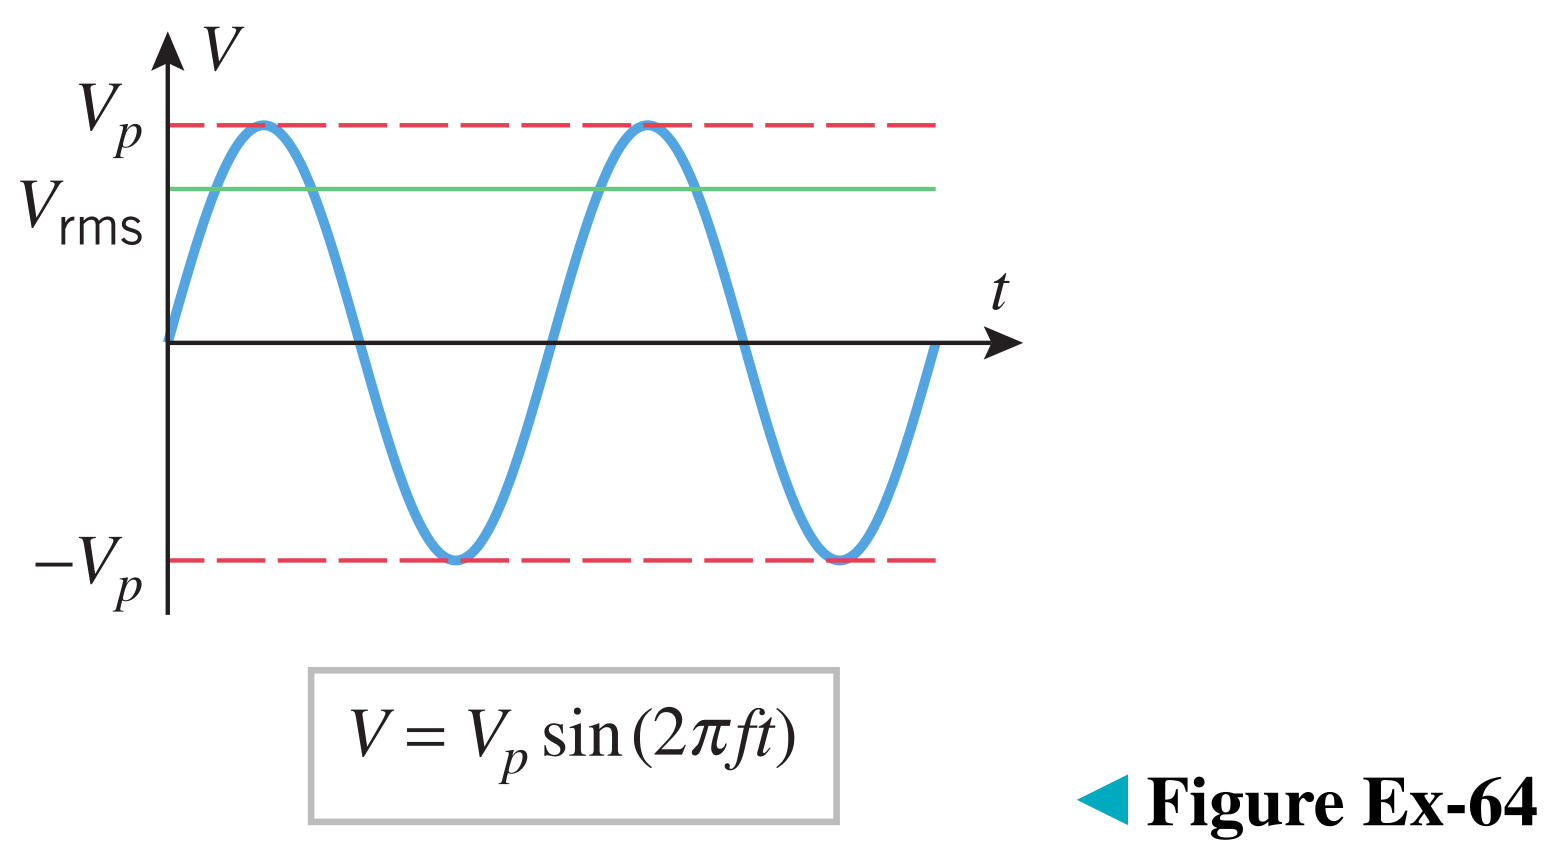
\includegraphics[width=0.7\textwidth]{../img/img_Lista4/1_64.png}
\end{figure}

La electricidad se suministra a los hogares en forma de \textbf{\textit{corriente alterna}}, lo que significa que el voltaje tiene una forma de onda sinusoidal descrita por una ecuación de la forma
\[
V = V_p \sin{(2\pi ft)}
\]
(ver la figura adjunta). En esta ecuación, $V_p$ se llama \textbf{\textit{voltaje máximo}} o \textbf{\textit{amplitud}} de la corriente, $f$ se llama \textbf{\textit{frecuencia}} y $1/f$ se llama \textbf{\textit{período}}. Los voltajes $V$ y $V_p$ se miden en voltios ($V$), el tiempo $t$ se mide en segundos ($s$) y la frecuencia se mide en hercios ($Hz$). ($1 Hz = 1$ ciclo por segundo; un \textbf{\textit{ciclo}} es el término eléctrico para un período de la forma de onda). La mayoría de los voltímetros de corriente alterna leen lo que se llama \textbf{\textit{rms}} o \textbf{\textit{valor cuadrático medio}} de $V$. Por definición, ésta es la raíz cuadrada del valor promedio de $V^2$ durante un período.
\begin{enumerate}[label=(\alph*)]
\item Demuestre que
  \[
  V_{rms}=\frac{V_p}{\sqrt{2}}
  \]
    [\textit{Sugerencia}: Calcule el promedio durante el ciclo de $t= 0$ a $t = 1/f$ y use la identidad $\sin^2{\theta}= \frac{1}{2}(1-\cos{2\theta})$ para ayudar a evaluar la integral.]

    Siguiendo la definición de los rms, tenemos que:

    \begin{align*}
      V_{rms}^2
      &= \frac{1}{\frac{1}{f}-0} \int_0^{\frac{1}{f}} \left[V_p^2 \sin^2{(2\pi ft)} \right] dt \\
      &= fV_p^2 \int_0^{\frac{1}{f}} \left[\sin^2{(2\pi ft)} \right] dt \\
      &= \frac{fV_p^2}{2} \int_0^{\frac{1}{f}} \left[ 1-\cos{(4\pi ft)} \right] dt 
    \end{align*}

  Si hacemos que $u = 4\pi ft$, entonces $u(\frac{1}{f})=4\pi$, $u(0)=0$ y
  
  \[
  \frac{du}{dt}=4\pi f \qquad \text{ así, } \qquad \frac{du}{4\pi f}=dt
  \]

  De este modo,

  \begin{align*}
    \frac{fV_p^2}{2} \int_0^{\frac{1}{f}} \left[ 1-\cos{(4\pi ft)} \right] dt 
    & =    \frac{fV_p^2}{2} \int_0^{4\pi} \left[ 1-\cos{u} \right] \frac{du}{4\pi f} \\
    & =    \frac{V_p^2}{8\pi} \int_0^{4\pi} \left[ 1-\cos{u} \right] du \\
    &= \frac{V_p^2}{8\pi} \left[ u-\sin{u} \right]_0^{4\pi}\\
    &= \frac{V_p^2}{8\pi} (4\pi-0)\\
    &=\frac{V_p^2}{2}
  \end{align*}

  Por lo que tenemos que $V_{rms}=\frac{V_p}{\sqrt{2}}$.
  
\item En Estados Unidos, los enchufes eléctricos suministran corriente alterna con un voltaje $rms$ de $120 V$ a una frecuencia de $60 Hz$. ¿Cuál es el voltaje máximo en tal toma corriente?

  \begin{align*}
    120V
    &= \frac{V_p}{\sqrt{2}} \\ \\
    \therefore V_p &= 120\sqrt{2}V \approx 169.705627 V
  \end{align*}


%Segunda parte de la lista de problemas
\subsection*{\centering \textbf{ \LARGE Segunda Parte} }
%% Sección 5.10: ejercicios 25, 26 y 27.
%% Sección 7.2: ejercicios 53, 54, 60 y 62.
  %% Sección 7.7: ejercicios 31, 32 y 34.
%% 5.10 -----------------------------------------------------------------------------------------------------------------------------------------------------------------------------------------------------------------------------
\section{Sección 5.10 \\Logaritmos y otras funciones definidas por integrales} 
% 25  -------------------------------------------------------------------------------------------------------------
\subsection{Ejercicio 25} Flores Morán Julieta Melina   \\
Usa los resultados del ejercicio 24 para encontrar la derivada: \\
Cabe poner a consideración que el ejercicio 24 pide demostrar las siguiente propiedades:
\[
\frac{d}{dx} \left[ \int_x^{a} f(t) dt \right] = -f(x)
\]
 \[
\frac{d}{dx} \left[ \int_{g(x)}^{a} f(t) dt \right] = -f(g(x))g'(x)
\]

\begin{enumerate}
\item
\[
\frac{d}{dx} \int_x^{\pi} cos(t^{3}}) dt
\]
Usaremos la primera propiedad, donde  $f(t) = cos(t^3) \rightarrow f(x) = cos(x^3)$.De aquí que:
\[
\frac{d}{dx} \int_x^{\pi} cos(t^{3}}) dt = -cos(x^3)
 \]
\item
\[
\frac{d}{dx} \int_{tanx}^{3} \frac{t^2}{1+t^2} dt
\]
Usaremos la segunda propiedad, donde  $f(t) =  \frac{t^2}{1+t^2} \rightarrow f(x) = \frac{x^2}{1+x^2} $ y $g(x) = \tan x$.De aquí que:
\begin{align*}
  \frac{d}{dx} \int_{tanx}^{3} \frac{t^2}{1+t^2} dt
  &=  -f(tanx) \frac{d}{dx} tanx \\
  &=  - \frac{tan^2x}{1+tan^2x} sec ^2 x \\
  &=  - \frac{tan^2x \cdot sec ^2 x }{1+tan^2x}  \\
  &=  - \frac{tan^2x \cdot sec ^2 x }{sec^2x}  \\
  &=  - tan^2x \\
\end{align*}
\end{enumerate}
  %% 26 --------------------------------------------------------------------------------------------------------------
  %% 27 ---------------------------------------------------------------------------------------------------------------
\subsection{Ejercicio 27} Flores Morán Julieta Melina \\
Encuentra
\[
\frac{d}{dx} \left[ \int_{3x}^{x^2} \frac{t-1}{t^2+1} dt \right]
\]
escribiendo
\[
\int_{3x}^{x^2} \frac{t-1}{t^2+1} dt = \int_{3x}^{0} \frac{t-1}{t^2+1} + \int_{0}^{x^2} \frac{t-1}{t^2+1} dt
\]
Entonces, podemos reescribir el problema de la siguiente manera:
\[
\frac{d}{dx} \left[ \int_{3x}^{x^2} \frac{t-1}{t^2+1} dt \right] = \frac{d}{dx} \left[\int_{3x}^{0} \frac{t-1}{t^2+1} dt\right]  + \frac{d}{dx} \left[ \int_{0}^{x^2} \frac{t-1}{t^2+1} dt \right]
\]
Podemos usar la propiedad
 \[
\frac{d}{dx} \left[ \int_{g(x)}^{a} f(t) dt \right] = -f(g(x))g'(x)
\]
Y para $\frac{d}{dx} \left[\int_{3x}^{0} \frac{t-1}{t^2+1} dt\right]$ podemos considerar $g(x) = 3x$, $f(t) = \frac{t-1}{t^2+1}$.

\begin{align*}
  \frac{d}{dx} \left[\int_{3x}^{0} \frac{t-1}{t^2+1} dt\right]
  & = - f(g(x))g'(x) \\
  & = - f(3x) \frac{d}{dx} 3x \\
  & = -  \frac{3x-1}{(3x)^2+1} \cdot 3 \\
  & = -  3 \cdot \frac{3x-1}{9x^2+1}
\end{end*}


Para $\frac{d}{dx} \left[ \int_{0}^{x^2} \frac{t-1}{t^2+1} dt \right]$, necesitamos que cumpla con las características para aplicar la propiedad de arriba. Esto lo logramos intercambiando los límites y cambiando el signo, así.
\[
 \int_{0}^{x^2} \frac{t-1}{t^2+1} dt = -  \int_{x^2}^{0} \frac{t-1}{t^2+1} dt
\]
Y
\[
\frac{d}{dx} \left[ \int_{0}^{x^2} \frac{t-1}{t^2+1} dt \right] = -\frac{d}{dx} \left[ \int_{x^2}^{0} \frac{t-1}{t^2+1} dt  \right]
\]
podemos considerar $g(x) = x^2$, $f(t) = \frac{t-1}{t^2+1}$.

\begin{align*}
  -\frac{d}{dx} \left[ \int_{x^2}^{0} \frac{t-1}{t^2+1} dt  \right]
  & = - (- f(g(x))g'(x)) \\
  & = f(x^2) \frac{d}{dx} x^2 \\
  & =   \frac{x^2-1}{(x^2)^2+1} \cdot 2x \\
  & = 2x \cdot \frac{x^2-1}{x^4+1}
\end{align*}

Así con estos resultados obtenemos que:
\begin{align*}
  \frac{d}{dx} \left[ \int_{3x}^{x^2} \frac{t-1}{t^2+1} dt \right]
  & =\frac{d}{dx} \left[\int_{3x}^{0} \frac{t-1}{t^2+1} dt\right]  + \frac{d}{dx} \left[ \int_{0}^{x^2} \frac{t-1}{t^2+1} dt \right] \\
  & = -  3 \cdot \frac{3x-1}{9x^2+1} + 2x \cdot \frac{x^2-1}{x^4+1}
\end{align*}
%% 7.2 -----------------------------------------------------------------------------------------------------------------------------------------------------------------------------------------------------------------------------
\section{Sección 7.2 \\Integración por partes} 
% 54  -------------------------------------------------------------------------------------------------------------
\subsection{Ejercicio 54} Flores Morán Julieta Melina  \\
Evaluá por partes la integral
\[
\int_0^{1} \frac{x^3}{\sqrt{x^2+1}}dx
\]
Usando:
\begin{enumerate}
\item Integración por partes\\
  Para usar la fórmula de integración por partes para esta integral definida
  \[
  \int_a^b u dv = uv \Bigg|_a^b - \int_a^b vdu
  \]
  Hay que elegir una u y una v. En este caso si $v=\sqrt{x^2+1} \rightarrow dv = \frac{x}{\sqrt{x^2+1}}dx$ y $u=x^2 \rightarrow du = 2xdx$ completa la integral que buscábamos. Usando la fórmula.
   \[
   \int_0^1 x^2  \frac{x}{\sqrt{x^2+1}} dx = x^2 \cdot \sqrt{x^2+1}  \Bigg|_0^1 - \int_0^1 \sqrt{x^2+1} \cdot 2xdx  \]

   La integral $\int_0^1 \sqrt{x^2+1} 2xdx $ es fácil obtenerla por sustitución. Si $u = x^2+1 \rightarrow du = 2x dx$. Así
   \begin{align*}
     \int_0^1 2x\sqrt{x^2+1} dx
     & = \int_{u(0)}^{u(1)} \sqrt{u} du\\
     & = \int_{1}^{2} u^{1/2} du\\
     & = \frac{2u^{3/2}}{3} \Bigg|_1^2\\
     & = \frac{2\cdot 2^{3/2}}{3} - \frac{2\cdot1^{3/2}}{3} \\
     & = \frac{4 \cdot \sqrt{2}}{3} - \frac{2}{3} \\
     & = \frac{4}{3}  \sqrt{2} - \frac{2}{3} \\
   \end{align}
   Entonces tenemos
   \begin{align*}
     x^2 \cdot \sqrt{x^2+1}  \Bigg|_0^1 - \int_0^1 \sqrt{x^2+1} \cdot 2xdx
     & =1^2 \cdot \sqrt{1^2+1} -[0^2 \cdot \sqrt{0^2+1} ] - [\frac{4}{3}  \sqrt{2} - \frac{2}{3}] \\
     & = 1 \cdot \sqrt{2}  - \frac{4}{3}  \sqrt{2} + \frac{2}{3} \\
     & =  -  \frac{1}{3} \sqrt{2}    + \frac{2}{3}
   \end{align*}
  
 \item Sustitución de $u= \sqrt{x^2+1}$ \\
   En este caso cabe tener en cuenta que $du = \frac{x}{\sqrt{x^2+1}}dx $
     \begin{align*}
       \int_0^{1} \frac{x^3}{\sqrt{x^2+1}}dx
       & = \int_{u(0)}^{u(1)} (u^2-1)du \\
       & = \int_{1}^{\sqrt{2}} (u^2-1)du \\
       & = \int_{1}^{\sqrt{2}} u^2 du - \int_{1}^{\sqrt{2}}  du \\
       & = \left (\frac{u^3}{3}  -  u \right) \Bigg|_1^{\sqrt{2}}\\
       & = \frac{\sqrt{2}^3}{3}  -  \sqrt{2} - \left[\frac{1^3}{3}  -  1 \right]\\
       & = \frac{2}{3}\sqrt{2}  -  \sqrt{2} - \frac{1}{3}  +  1\\
       & = -\frac{1}{3}\sqrt{2} + \frac{2}{3}  \\
   \end{align*}
\end{enumerate}
% 62  -------------------------------------------------------------------------------------------------------------
\subsection{Ejercicio 62} Flores Morán Julieta Melina  \\
Usa la formula (9)
\[
\int \cos^n dx = \frac{1}{n}\cos^{n-1}x \sin x+\frac{n-1}{n} \int cos^{n-2}x dx
\]
de reducción para evaluar
\begin{enumerate}
\item
\[
  \int cos^5x dx
  \]

  Para esto necesitamos el valor de $\int cos^{3}x dx$.
  \begin{align*}
   \int  cos^3x dx
   & = \frac{1}{3}\cos^{2}x \sin x+\frac{2}{3} \int cos^{1}x dx \\
   & = \frac{1}{3}\cos^{2}x \sin x+\frac{2}{3} senx + C
  \end{align*}
  Así que volviendo al problema original
   \begin{align*}
    \int cos^5x dx
    & = \frac{1}{5}\cos^{4}x \sin x+\frac{4}{5} \int cos^{3}x dx\\
    & = \frac{1}{5}\cos^{4}x \sin x+\frac{4}{5} \left[\frac{1}{3}\cos^{2}x \sin x+\frac{2}{3} \sen x \right]\\
     & = \frac{1}{5}\cos^{4}x \sin x+ \frac{4}{15}\cos^{2}x \sin x+\frac{8}{15} \sen x + C
  \end{align*}
\item
 \[
  \int_0^{\frac{\pi}{2}} cos^6x dx
  \]
  Evaluaremos primero $ \int cos^6x dx$, para lo cual necesitamos conocer
  \begin{align*}
   \int  cos^2x dx
   & = \frac{1}{2}\cos^{1}x \sin x+\frac{1}{2} \int cos^{0}x dx \\
   & = \frac{1}{2}\cos^{1}x \sin x+\frac{1}{2} \int dx \\
   & = \frac{1}{2}\cos x \sin x+\frac{1}{2} x + C \\
  \end{align*}
  
  \begin{align*}
   \int  cos^4x dx
   & = \frac{1}{4}\cos^{3}x \sin x+\frac{3}{4} \int cos^{2}x dx \\
   & = \frac{1}{4}\cos^{3}x \sin x+\frac{3}{4} \left[ \frac{1}{2}\cos x \sin x+\frac{1}{2} x \right]\\
    & = \frac{1}{4}\cos^{3}x \sin x+ \frac{3}8\cos x \sin x+\frac{3}{8} x + C\\
  \end{align*}
  Y ya podemos resolver fácilmente para n=6.
  \begin{align*}
   \int  cos^6x dx
   & = \frac{1}{6}\cos^{5}x \sin x+\frac{5}{6} \int cos^{4}x dx \\
   & = \frac{1}{6}\cos^{5}x \sin x+\frac{5}{6} \left[ \frac{1}{4}\cos^{3}x \sin x+ \frac{3}8\cos x \sin x+\frac{3}{8} x  \right]\\
   & = \frac{1}{6}\cos^{5}x \sin x+ \frac{5}{24}\cos^{3}x \sin x+ \frac{15}{48}\cos x \sin x+\frac{15}{48} x \\
   & = \frac{1}{6}\cos^{5}x \sin x+ \frac{5}{24}\cos^{3}x \sin x+ \frac{5}{16}\cos x \sin x+\frac{5}{16} x + C \\
   \end{align*}
    Ahora hay que evaluarlo en los límites dados
    \begin{align*}
   \int_0^{\frac{\pi}{2}}cos^6x dx
   & = \left [\frac{1}{6}\cos^{5}x \sin x+ \frac{5}{24}\cos^{3}x \sin x+ \frac{5}{16}\cos x \sin x+\frac{5}{16} x \right] \Bigg|_0^{\frac{\pi}{2}}\\
   & =  \frac{1}{6}\cos^{5}  \left( \frac{\pi}{2} \right) \sin \left( \frac{\pi}{2} \right)+ \frac{5}{24}\cos^{3}\left( \frac{\pi}{2} \right) \sin \left( \frac{\pi}{2} \right)  \\
     & + \frac{5}{16}\cos \left( \frac{\pi}{2} \right) \sin \left( \frac{\pi}{2} \right)+\frac{5}{16} \left( \frac{\pi}{2} \right)\\
   &  - \left [\frac{1}{6}\cos^{5} 0 \sin 0+ \frac{5}{24}\cos^{3}0 \sin 0+ \frac{5}{16}\cos 0 \sin 0+\frac{5}{16} 0 \right] \\
   & = \frac{5}{16} \left( \frac{\pi}{2} \right) \\
   & = \frac{5 \pi}{32}
   \end{align*}
\end{enumerate}
%% 7.7 -----------------------------------------------------------------------------------------------------------------------------------------------------------------------------------------------------------------------------
\section{Sección 7.7 \\Integración numérica: Regla de Simpson} 
% 32  -------------------------------------------------------------------------------------------------------------
\subsection{Ejercicio 32} Flores Morán Julieta Melina  \\
El valor exacto de la integral dada es $\pi$ (verificar). Aproximar la integral usando (a) la aproximación del punto medio$ M_{10}$, (b) la aproximación trapezoidal $T_{10}$, y (c) Aproximación de la regla de Simpson $ S_{20}$ usando la Fórmula (7). Aproximar el error absoluto y expresa tus respuestas con al menos cuatro decimales.
\[
\int_0^3 \frac{4}{9} \sqrt{9-x^2} dx
\]
\begin{enumerate}
\item Verificar el valor de la integral dada, esta es una integral del formulario, entonces usamos la formula.
   \begin{align*}
     \int_0^3 \frac{4}{9} \sqrt{9-x^2} dx
     & = \frac{4}{9}  \int_0^3 \sqrt{9-x^2} dx \\
     & = \frac{4}{9}  \left[ \frac{x}{2} \sqrt{9-x^2} + \frac{9}{2} \sin ^{-1} {\frac{x}{3}} \right] \Bigg|_0^3  \\
     & = \left[ \frac{4x}{18} \sqrt{9-x^2} + \frac{36}{18} \sin^{-1} {\frac{x}{3}}\right]  \Bigg|_0^3   \\
     & = \left[ \frac{2x}{9} \sqrt{9-x^2} + 2 \sin^{-1} {\frac{x}{3}} \right] \Bigg|_0^3  \\
     & = \left[ \frac{2 \cdot 3}{9} \sqrt{9-3^2} + 2 \sin^{-1} {\frac{3}{3}} \right] - \left[ \frac{2 \cdot 0}{9} \sqrt{9-0^2} + 2 \sin^{-1} {\frac{0}{3}} \right] \\
     & = \left[ \frac{2}{3} \sqrt{9-9} + 2 \sin^{-1} {1} \right] - \left[  2 \sin^{-1} {0} \right] \\
     & = \left[ 2 \cdot \frac{\pi}{2} \right] - \left[  2 \cdot 0 \right] \\
     & = \pi
   \end{align*}
 \item Aproximar la integral
   \begin{enumerate}
   \item $M_{10}$ \\
     Este método se describe de la siguiente forma:
     \[
     M_n = \left( \frac{b-a}{n} \right) \sum_{k=1}^{n}f(x_k^*)
     \]
     \[
     x_k^* = \frac{1}{2}(x_{k-1} + x_k)
     \]
     \begin{figure}[H]
       \centering
       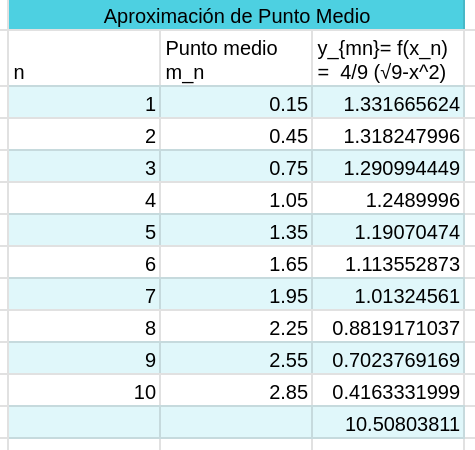
\includegraphics[width=0.7\textwidth]{../img/img_Lista4/MP.png}
     \end{figure}
     \[
      M_{10} =  (0.30)(10.0803811)= 3.152411433
     \]
   \item $T_{10}$ \\
     Usaremos la definición que dice que
     \[
     T_n = \left( \frac{b-a}{2n}\right)[y_0 + 2y_1 + \ldots +2 y_{n-1} + y_n]
     \]
     \begin{figure}[H]
       \centering
       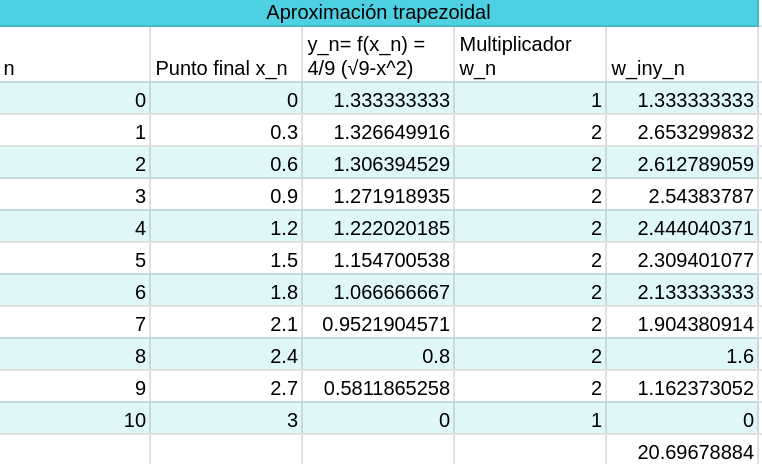
\includegraphics[width=0.7\textwidth]{../img/img_Lista4/TN1.png}
     \end{figure}
      \[
      T_{10} =  (0.15)(20.69678884)= 3.104518326
      \]
      
   \item $S_{20}$ \\
     Este método se basa en los anteriores y se describe como sigue
     \[
     S_n = S_{2k} = \frac{1}{3} (2M_k + T_k)
     \]
     En este caso tenemos que con lo ya calculado:
     \[
     S_{20} = S_{2 ~10} = \frac{1}{3} (2M_{10} + T_{10})
     \]
      \[
     S_{20} = 3.136447064
     \]
    \end{enumerate}
 \item Error absoluto
    \begin{enumerate}
   \item $|M_{10}| = |\pi - M_{10}| \approx |-0.010807| = 0.010807$
   \item $|T_{10}|  = |\pi - T_{10}| \approx |0.0370926| = 0.0370926 $
    \item $|S_{20}|  = |\pi - S_{20}| \approx |0.0051455| = 0.0051455 $
   \end{enumerate}
\end{enumerate}

%Tercera parte de la lista de problemas
\subsection*{\centering \textbf{ \LARGE Tercera Parte} }
%% Sección 6.1: ejercicios 17, 31, 38 y 42.
%% Sección 6.6: ejercicios 8, 17 y 22.
%% Sección 7.8: ejercicios 7, 28 y 39.

%% 6.1 -----------------------------------------------------------------------------------------------------------------------------------------------------------------------------------------------------------------------------
\section{Sección 6.1 \\Área entre dos curvas}
% 17  -------------------------------------------------------------------------------------------------------------
\subsection{Ejercicio 17} Flores Morán Julieta Melina  \\
Dibuja la región entre las curvas y encuentra su área.
\[
y = 2 + |x-1|, y=-\frac{1}{5}x + 7
\]
$y = 2 + |x-1|$ : Esta es la función del valor absoluto desplazada dos unidades hacia arriba y una a la derecha.\\
$y=-\frac{1}{5}x + 7 $: Esta es una línea recta que intersecta al eje y en 7 y al eje x en 35.\\
Para conocer el intervalo de integración debemos encontrar los puntos de intersección.
Por $y=-\frac{1}{5}x + 7$, $x = 35-5y$ \\
Entonces sustituimos en y = 2 + |x-1|\\
\begin{align*}
  y 
  & = 2 + |x-1|\\
  & = 2 + | 35-5y-1| \\
  & = 2 + |34-5y|
\end{align*}
Como nos encontramos con el valor absoluto hay dos puntos de intersección donde se satisface la ecuación.
\begin{align*}
  y_1 = 
  & = 2 + 34-5y_1 \\
  & = 36-5y_1
\end{align*}
\begin{align*}
  6y_1= 36
\end{align*}
\begin{align*}
  y_1= 6
\end{align*}
Para este valor, remplazamos en $x = 35-5y$
\begin{align*}
  x =
  & = 35-5(6) \\
  & = 35-30 \\
  & = 5
\end{align*}
Así que hay un punto de intersección en $(5,6)$\\
Ahora usamos el otro valor que puede tomar y.\\
\begin{align*}
  y_2 = 
  & = 2  - 34 + 5y_2 \\
  & = -32 + 5y_2
\end{align*}
\begin{align*}
  4y_2= 32
\end{align*}
\begin{align*}
  y_2= 8
\end{align*}
Para este valor, remplazamos en $x = 35-5y$
\begin{align*}
  x =
  & = 35-5(8) \\
  & = 35-40 \\
  & = -5
\end{align*}
Así que hay un punto de intersección en $(-5,8)$\\
Con esta información podemos dibujar estas gráficas.
\begin{figure}[H]
       \centering
       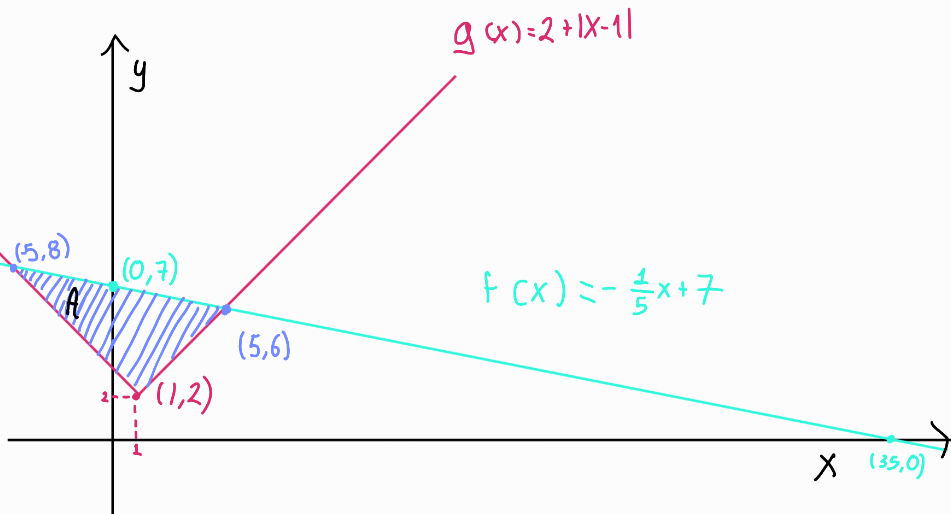
\includegraphics[width=0.7\textwidth]{../img/img_Lista4/gra17.png}
\end{figure}
Estamos buscando el área en morado. Para facilitar esto, podemos entender $y = 2 + |x-1|$ como  $g(x)= \left\{ \begin{array}{lcc} 1+x & si & x>1 \\ \\ 3-x & si & x<1 \\ \end{array} \right. $. \\\\
El área entre estas rectas, donde $f(x) \geq g(x)$ en $[-5,5]$ esta dada por la fórmula:
\[
A = \int_{-5}^5 [f(x)-g(x)] dx
\]
Si separamos el área en dos partes desde -5 a 1 y de 1 a 5 podremos calcularlas con las rectas que le corresponden según la definición anterior de g(x)
Así que tenemos que:
\[
A = \int_{-5}^1 [f(x)-g(x)] dx + \int_{1}^5 [f(x)-g(x)]
\]
\begin{align*}
  A
  & =  \int_{-5}^1 \left[ \left( \frac{-x}{5} + 7 \right) - \left( 3-x \right) \right] dx + \int_{1}^5 \left[ \left( \frac{-x}{5} + 7 \right)- \left( x+1 \right) \right] dx\\
  & =  \int_{-5}^1 \left[  \frac{-x}{5} + 7  - 3 + x  \right] dx + \int_{1}^5 \left[  \frac{-x}{5} + 7 - x - 1  \right] dx\\
  & =  \int_{-5}^1 \left[  \frac{-4x}{5} + 4   \right] dx + \int_{1}^5 \left[  \frac{-6x}{5} + 6   \right] dx\\
  & = \frac{4}{5} \int_{-5}^1 x dx  + \int_{-5}^1 4   dx - \frac{6}{5}  \int_{1}^5 x dx  +  \int_{1}^5 6  dx\\
  & = \frac{4}{5} \left[ \frac{x^2}{2} \Big|_{-5}^1 \right]  +  4x\Big|_{-5}^1    - \frac{6}{5}  \left[ \frac{x^2}{2} \Big|_{1}^5 \right]  +   6x \Big|_{1}^5\\
  & = \frac{4}{5} \left[ \frac{1}{2} - \frac{25}{2}  \right]  +  4(1+5)   - \frac{6}{5}  \left[ \frac{25}{2} - \frac{1}{2}  \right]  +   6 (5-1)\\
  & = \frac{4}{5} \left[ -\frac{24}{2}  \right]  +  4(6)   - \frac{6}{5}  \left[ \frac{24}{2} \right]  +   6 (4)\\
  & =  -\frac{96}{10}  +  24   -  \frac{144}{10}   +   24\\
  & =  -\frac{240}{10}  +  48 = 24\\
\end{align*}
% 31  -------------------------------------------------------------------------------------------------------------
% 38  -------------------------------------------------------------------------------------------------------------
\subsection{Ejercicio 38} Flores Morán Julieta Melina  \\
Encuentra el área entre las curvas y = sen x y el segmento de línea uniendo los puntos (0,0) y (5$\pi$/6, 1/2) de la curva. \\

Para encontrar la fórmula de la recta que une a los puntos dados, podemos usar la ecuación de la recta $y - y_1 = m (x-x_1)$, donde $m=\frac{\frac{1}{2} - 0}{ \frac{5\pi}{6} - 0}$.\\
Así que tenemos que $ y- 0 = m (x-0)$ resulta en la formula deseada.
\[
y = \frac{6}{10\pi} x = \frac{3}{5\pi} x
\]
Ahora, ya que la función $ y=senx \geq y= \frac{3}{5\pi} x $, usamos la fórmula para el área de la siguiente manera:
\begin{align*}
  A =
  & = \int_{0}^{\frac{5\pi}{6}} \left[  senx -  \frac{3}{5\pi} x \right]dx\\
  & = \int_{0}^{\frac{5\pi}{6}}   senx dx -  \int_{0}^{\frac{5\pi}{6}} \frac{3}{5\pi} x dx \\
  & = -cosx \Big|_{0}^{\frac{5\pi}{6}} -   \frac{3}{5\pi}  \int_{0}^{\frac{5\pi}{6}} x dx\\
  & = -(cos \frac{5\pi}{6} - cos0 ) -   \frac{3}{5\pi} (\frac{x^2}{2}\Big|_{0}^{\frac{5\pi}{6}} )\\
  & = -(cos \frac{5\pi}{6} - cos0 ) -   \frac{3}{5\pi} (\frac{x^2}{2}\Big|_{0}^{\frac{5\pi}{6}} )\\
  & = -( - \frac{\sqrt{3}}{2} - 1) - \frac{3}{5\pi} (\frac{ (\frac{5\pi}{6})^2 }{2} )  \\
  & = \frac{2+ \sqrt{3}}{2} - \frac{\frac{75 \pi  ^2}{36}}{10\pi} \\
  & = \frac{2+ \sqrt{3}}{2} - \frac{75 \pi  ^2}{360\pi} \\
  & = \frac{2+ \sqrt{3}}{2} - \frac{5 \pi}{24} \\
 \end{align*}
% 42  -------------------------------------------------------------------------------------------------------------
%% 6.6 -----------------------------------------------------------------------------------------------------------------------------------------------------------------------------------------------------------------------------
\section{Sección 6.6 \\Trabajo}
% 8  -------------------------------------------------------------------------------------------------------------
\subsection{Ejercicio 8} Flores Morán Julieta Melina  \\}
Un resorte cuya longitud natural es de 15 cm ejerce una fuerza de
45 N cuando se estira hasta una longitud de 20 cm.
\begin{enumerate}
\item Encuentre la constante del resorte (en newtons/metro). \\
Sabemos que $F(x) = k*x$ y por el enunciado inicial deducimos que la fuerza utilizada para estirar el resorte 5 cm es de 45 N. $F(0.05) = 45 N = k(0.05)$. Por esto $k = \frac{45 N}{0.05 m} = 900 N/m$
\item  Encuentre el trabajo que se realiza al estirar el resorte 3 cm.
  más allá de su longitud natural.\\
  Considerando que $W = \int_a^b F(x)dx$. Basta con especificar que los limites de integración será de 0 m de estiramiento a 0.03 m de estiramiento.

  \begin{align*}
    W
    & = \int_0^{0.03} 900x dx \\
    & = 900 \int_0^{0.03} x dx \\
    & = 900 \left[ \frac{x^2}{2} \Big|_0^{0.03} \right] \\
    & = 900 \left[ \frac{(0.03)^2}{2} - 0  \right]\\
    & = 900 \left[ 0.00045  \right] \\
    & = 0.405 J \\
  \end{align*}
\item Encuentre el trabajo realizado al estirar el resorte desde una longitud de 20 cm hasta una longitud de 25 cm. \\
  Aplicaremos la misma lógica del inciso b), excepto que esta vez nuestros límites de integración van desde 0.05 m de estiramiento hasta 0.1 m de estiramiento.
  \begin{align*}
    W
    & = \int_{0.05}^{0.1} 900x dx \\
     & = 900 \int_{0.05}^{0.1} x dx \\
    & = 900 \left[ \frac{x^2}{2} \Big|_{0.05}^{0.1} \right] \\
    & = 900 \left[ \frac{(0.1)^2}{2} -  \frac{(0.05)^2}{2}  \right]\\
    & = 900 \left[ 0.005 - 0.00125  \right]\\
    & = 900 \left[ 0.00375  \right] \\
    & = 3.37 J \\
  \end{align*}
  
\end{enumerate}

% 17  -------------------------------------------------------------------------------------------------------------
% 22  -------------------------------------------------------------------------------------------------------------
%% 7.8 -----------------------------------------------------------------------------------------------------------------------------------------------------------------------------------------------------------------------------
\section{Sección 7.8 \\Integrales impropias}
% 7  -------------------------------------------------------------------------------------------------------------
\subsection{Ejercicio 7} Flores Morán Julieta Melina  \\
Evaluá las integrales que convergen:
\[
\int_{e}^{+\infty} \frac{1}{xln^3 x} dx
\]
Usando la fórmula general para una integral impropia en el intervalo [a, $+ \infty$].
\[
\int_{e}^{+\infty} \frac{1}{xln^3 x} dx = \lim_{b \to \infty} \int_{e}^{b} \frac{1}{xln^3 x} dx 
\]
Primero encontramos la integral mediante sustitución donde $u=lnx \rightarrow du = \frac{1}{x}dx$
  \begin{align*}
    \int_{e}^{b} \frac{1}{xln^3 x} dx 
    & = \int_{u(e)}^{u(b)} \frac{1}{ u^3} du  \\
     & = \int_{1}^{lnb} u^{-3} du  \\
      & = \frac{u^{-2}}{-2} \Big|_{1}^{lnb}\\
      & =- \frac{1}{2 u ^2} \Big|_{1}^{lnb} \\
    & = \left[ -\frac{1}{2  (lnb)^2}] - [-\frac{1}{2 \cdot 1 ^2} \right]  \\
     & =\left[ \frac{1}{2} -\frac{1}{2  (lnb)^2} \right]   \\
  \end{align*}
  Ahora evaluemos:
  \begin{align*}
    \lim_{b \to \infty} \int_{e}^{b} \frac{1}{xln^3 x} dx 
    & =  \lim_{b \to \infty}   \left[ \frac{1}{2} -\frac{1}{2  (lnb)^2} \right]  \\
    & = \frac{1}{2} -0 = \frac{1}{2}
  \end{align*}
 % 28  -------------------------------------------------------------------------------------------------------------

% 39  -------------------------------------------------------------------------------------------------------------
\subsection{Ejercicio 39} Flores Morán Julieta Melina  \\
Usa sustitución y evaluá la integral resultante indefinida
\[
\int_{0}^{+\infty} \frac{e^{-x}}{\sqrt{1-e^{-x}}}dx
\]
\[
u = 1-e^{-x}
\]
Nota: $u \rightarrow 1$ mientras que $x \rightarrow + \infty$\\ \\
Evaluemos primero la integral con límite superior b donde $du = e^{-x}dx$
  \begin{align*}
    \int_{0}^{+\infty} \frac{e^{-x}}{\sqrt{1-e^{-x}}}dx
    & = \lim_{b \to + \infty} \int_{0}^{b} \frac{e^{-x}}{\sqrt{1-e^{-x}}}dx   \\
    & = \lim_{b \to + \infty} \int_{u(0)}^{u(b)} \frac{du}{\sqrt{u}}   \\
    & = \lim_{b \to + \infty} \int_{0}^{1-e^{-b}} u^{\frac{-1}{2}} du\\
    & = \lim_{b \to + \infty} \left[ \frac{u^{\frac{1}{2}}}{\frac{1}{2}} \Big|_0^{1-e^{-b}} \right]\\
    & = \lim_{b \to + \infty} \left[ 2u^{\frac{1}{2}}\Big|_0^{1-e^{-b}} \right]\\
    & = 2\lim_{b \to + \infty} \left[u^{\frac{1}{2}}\Big|_0^{1-e^{-b}} \right]\\
    & = 2\lim_{b \to + \infty} \left[ \sqrt{1-e^{-b}} - \sqrt{0}  \right]\\
    & = 2\lim_{b \to + \infty} \left[ \sqrt{1-e^{-b}} \right]\\
    & = 2  \left[ \sqrt{1-0} \right]\\
    & = 2 \\
  \end{align*}
\end{document}

                              
